\documentclass[12pt, a4paper, titlepage]{article}
\usepackage[spanish]{babel}
\usepackage[utf8]{inputenc}
\usepackage{float}
\usepackage{subfig}
%%Imágenes
\usepackage{graphicx}
%%Colores de texto 
\usepackage{xcolor}
\usepackage{colortbl}
%%Links
\usepackage[hidelinks]{hyperref}
%%Comentarios
\usepackage{verbatim}

%---------------------------GLOSARIO----------------------------%
\usepackage{glossaries}
\makeglossaries

\newglossaryentry{Flash}
{
    name=Flash,
    description={Aplicación informática englobada en la categoría de reproductor multimedia}
}
\newglossaryentry{NetScape}{
    name=Netcape,
    description={Navegador web de la compañia NetScape Communications}
}
\newglossaryentry{cookies}{
    name=Cookies,
    description={Es una pequeña información enviada por un sitio web y almacenada en el navegador del usuario, de manera que el sitio web puede consultar la actividad previa del navegador.
    Sus principales funciones son recordar accesos y
    conocer información sobre los hábitos de navegación e intentos de spyware}
}

\newglossaryentry{HMACSHA14}{
    name=HMACSHA14,
    description={HMAC-SHA1 es un tipo de algoritmo o herramienta que provee un algoritmo estandar MAC.}
}

\newglossaryentry{backdoor}{
    name=Backdoor,
    description={Una puerta trasera o backdoor es una secuencia especial dentro del código de programación, mediante la cual se pueden evitar los sistemas de seguridad del algoritmo (autenticación) para acceder al sistema. Aunque estas puertas pueden ser utilizadas para fines maliciosos y espionaje no siempre son un error, ya que pueden haber sido diseñadas con la intención de tener una entrada secreta}
}

\newglossaryentry{Robo de Identidad}{
    name=Identity theft,
    description={También conocido como ''robo de identidad'' se produce cuando una persona adquiere, transfiere, posee o utiliza información personal de una persona física o jurídica de forma no autorizada, con la intención de efectuar o vincularlo con algún fraude u otro delito}
}
%\acrlong{}  \acrshort{} 
\newacronym{html}{HTML}{Hyper Text Markup Languaje}
\newacronym{iu}{IU}{Interfaz de Usuario}
\newacronym{http}{HTTP}{Hypertext Transfer Protocol}
\newacronym{css}{CSS}{Cascading Style Sheets}
\newacronym{url}{URL}{Uniform Resource Locator}

%------------------FINAL DE GLOSARIO-----------------------%
%------------------ESTABLECER COLORES----------------------%
\definecolor{guindapoli}{RGB}{102, 0, 51}
\definecolor{azulescom}{RGB}{0, 0, 102}
\definecolor{azulclaro}{RGB}{222, 232, 255}
\definecolor{azulfuerte}{RGB}{60, 150, 250}
%------------------FIN DE COLORES------------------%
\begin{document}
	
	%PORTADA
	\begin{titlepage}	
		
		\vspace*{-1.5in}
		
		\begin{figure}[htb]
	    \begin{minipage}{0.5\textwidth}
        %    \centering
            
\includegraphics[width=0.8\textwidth]{imagenes/logoipn.png}
        \end{minipage}%
        \hspace{5mm}
        \begin{minipage}{0.5\textwidth}
        %    \centering
            
\includegraphics[width=0.8\textwidth]{imagenes/logoescom.png}
        \end{minipage}
		\end{figure}
		
		\begin{center}
			
			\begin{LARGE}
				\textcolor{guindapoli}{INSTITUTO POLITÉCNICO NACIONAL}\\
			\end{LARGE}	
			
			\vspace*{0.2in}
			
			\begin{Large}
				\textcolor{azulescom}{ESCUELA SUPERIOR DE CÓMPUTO}\\
			\end{Large}		
			
			\vspace*{0.4in}
			
			\begin{large}
				Trabajo Terminal I.\\
			\end{large}
			
			\vspace*{0.2in}
			
			\begin{Large}
				\textbf{Autentificación mediante Chaffing and Winnowing en el protocolo HTTP}\\
			\end{Large}
			
			\vspace*{0.2in}
			
			\begin{large}
				2018-B003.\\
			\end{large}
			
			\vspace*{0.2in}
			
			\rule{80mm}{.1mm}\\
			\vspace*{0.1in}
			
			\begin{large}
				\begin{center}
					Integrantes:\\
					Carrillo Fernández Gerardo\\
					Blancas Pérez Bryan Israel\\
					Morales González Diego Arturo\\
					Paredes Hernández Pedro Antonio\\
				\end{center}
			\end{large}
			
			\begin{large}
				Directores:\\
				Moreno Cervantes Axel Ernesto\\
				Díaz Santiago Sandra\\
			\end{large}
			
		\end{center}
	
	\end{titlepage}
    %Índice
	\begin{appendix}
		\renewcommand*\contentsname{{\textcolor{azulescom}{Índice.}}}
		\tableofcontents
		\newpage
		%%índice de figuras
		\renewcommand*\listfigurename{{\textcolor{azulescom}{Índice de figuras.}}}
		\listoffigures
		\newpage
		%%Índice de tablas
		\newpage
		\renewcommand*\listtablename{{\textcolor{azulescom}{Índice de cuadros.}}}
		\listoftables
		
		\newpage
		\renewcommand*\glossaryname{{\textcolor{azulescom}{Glosario.}}}
		
		\printglossary
	\end{appendix}
	\newpage
	
	\textbf{\textcolor{azulescom}{\Huge{Capítulo 1.}}}

	\renewcommand\thesection{\arabic{section}}	
	\section{\textcolor{azulescom}{Introducción.}}
		
		En la actualidad la mayor\'ia de los usuarios de internet necesitan guardar contraseñas para sus distintas cuentas en las diferentes páginas web a las que ingresan, ya que recordarlas es un problema debido a la gran cantidad de servicios que se utilizan en la actualidad. Como consecuencia de que la autentificaci\'on por contraseña es la más utilizada en los servicio web hoy en día \cite{ComparisonAuthenticationMethodsResources}, los distintos servicios web han implementado mecanismos de seguridad tales como contraseñas que contengan un mínimo de carateres determinados, al menos un caracter especial, entre otros. Esto ha provocado que éstas sean más difíciles de recordar y han orillado a los usuarios a optar por guardarlas en medios físicos o digitales para recordarlas cuando sea necesario. 
		Sin embargo, perder esas claves (principalmente con los medios físicos) presenta un grave problema de seguridad, teniendo como consecuencia: perdida de datos sensibles, robo de identidad, robo de cuentas bancarias, etc.\\
		
		La gran mayoría de servicios web han implementado la función "recordar contraseña", la cual hace que el usuario no tenga que ingresar sus credenciales\footnote{Credenciales se entiende como los datos que un servicio web requiere para poder acceder al él. Comúnmente son 'usuario' y 'contraseña'.} cada vez que se quiere acceder al servicio. Esta función por lo general hace uso de cookies cuyas vulnerabilidades se explicarán más adelante.
	    
		Es por ello, que en este trabajo terminal, propone un nuevo método de autentificación por medio de \textit{Chaffing and Winnowing} y con la ayuda de una extensión de Google Chrome, la cual servirá para la inyección de las credenciales de la autentificación del usuario en el protocolo \acrshort{http}. Así, si un servicio web tiene este tipo de autentificación disponible, lo podrá validar. El propósito principal de este trabajo es que los usuarios puedan realizar un inicio de sesión más cómodo, seguro y sin la necesidad de recordar sus distintas contraseñas.
		
		\newpage
			
		\subsection{Objetivos.}
			\subsubsection{Objetivo general. }
			Realizar una extensión en Google Chrome que modifique los datos del protocolo \acrshort{http}, para permitir que el servidor detecte el método de autentificación propuesto basado en \textit{Chaffing and Winnowing}.\\
			\subsubsection{Objetivos particulares.}
			\begin{itemize}
				\item Investigar e implementar el desarrollo de extensiones en Google Chrome.
				\item Investigar sobre los mecanismos de autentificación.
				\item Investigar sobre la técnica de \textit{Chaffing and Winnowing} para adaptar su implementación.
				\item Inyectar el código (la autentificación) en el encabezado HTTP para enviar la petición al servidor. 
				\item Modificar el código del servidor Apache para simular y comprobar el funcionamiento de la extensión.
				\item Realizar pruebas de seguridad para comprobar la eficacia de la extensión. 
			\end{itemize}
		\subsection{Metodolog\'ia.}
		El proceso de desarrollo que seguiremos estará basado en la metodología de prototipos evolutivos, el cual consiste en la implementación parcial del proyecto cumpliendo con los requerimientos que van surgiendo a lo largo del desarrollo , de esta manera es posible ir experimentando con un prototipo parcialmente funcional e identificar posibles mejoras o fallas con el fin de lograr el objetivo final.
		Esta metodología está compuesta por las siguientes fases:
		\begin{itemize}
		    \item Fase de investigación preliminar.
		    \item Especificación de requerimientos y prototipos
		    \item Diseño técnico
		    \item Programación y pruebas
		    \item Operación y mantenimiento
		\end{itemize}
		
        
        Primero tendremos la fase de “investigación preliminar”, donde se van a definir las metas principales, después en la fase de “especificación de requerimientos y prototipos", se hace el diseño básico para dar paso a la creación del primer prototipo correspondiente, y después verificar el cumplimiento de los requerimientos y de ser necesario modificarlo hasta que los cumpla. En la tercera fase (diseño técnico) se realiza un diseño detallado y la documentación necesaria para que en la cuarta fase (programación y pruebas) se implemente y se pruebe el prototipo. Finalmente, en la última fase (Operación y mantenimiento) se hace la liberación y el mantenimiento del prototipo final.
        
        Para nuestro proyecto realizaremos 4 prototipos, los cuales son: 
        \begin{enumerate}
            \item Creación de extensión de Google Chrome para interceptar la petición \acrshort{http}. 
            \begin{itemize}
                \item Investigación preliminar: 
                \begin{itemize}
                    \item Investigar sobre el desarrollo de extensiones en Google Chrome.
                \end{itemize}
                \item Especificación de requerimientos y prototipos:
                \begin{itemize}
                    \item Ejecución de la extensión sobre Google Chrome.
                    \item Detectar petición \acrshort{http} e interceptarla.
                    \item Subir archivo autentificador a la extensión.
                \end{itemize}
                \item Diseño técnico: 
                \begin{itemize}
                    \item Documentación del prototipo.
                \end{itemize}
                \item Documentación del prototipo.
                \begin{itemize}
                    \item Desarrollo de la extensión.
                    \item Pruebas de la extensión.
                \end{itemize}
            \end{itemize}
            \item Inyección de código autentificador (Chaffing) en el encabezado \acrshort{http}. 
            \begin{itemize}
                \item Investigación preliminar: 
                \begin{itemize}
                    \item Investigación sobre el método Chaffing and Winnowing. 
                \end{itemize}
                \item Especificación de requerimientos y prototipos: 
                \begin{itemize}
                    \item  Lectura del archivo autentificador.
                    \item  Análisis del protocolo \acrshort{http}. 
                    \item  Inyección del código autentificador sobre el protocolo \acrshort{http}.
                    \item Mandar petición a servidor.
                \end{itemize}
                \item Diseño técnico:
                \begin{itemize}
                    \item Documentación del prototipo. 
                \end{itemize}
                \item Programación y pruebas: 
                \begin{itemize}
                    \item Desarrollo del complemento de la extensión. 
                    \item Creación del algoritmo de inyección de código. 
                    \item Pruebas de la extensión. 
                \end{itemize}
            \end{itemize}
            \item Modificación del servidor Apache para recibir el protocolo con la inyección de código.
            \begin{itemize}
                \item  Investigación preliminar: 
                \begin{itemize}
                    \item Investigación sobre el servidor Apache.
                    \item Analizar la arquitectura del servidor Apache
                    \item Investigación sobre la versión conveniente a modificar.
                \end{itemize}
                \item Especificación de requerimientos y prototipos: 
                \begin{itemize}
                    \item Recibir petición \acrshort{http} de la extensión. 
                    \item  Detectar el tipo de autentificación que se usará.
                \end{itemize}
                \item Diseño técnico: 
                \begin{itemize}
                    \item Documentación del prototipo.
                \end{itemize}
                \item Programación y pruebas:
                \begin{itemize}
                    \item Descargar la versión del servidor Apache a usar.
                    \item Modificación del código del servidor Apache para detectar el tipo de autentificación que se usará. 
                    \item Pruebas de funcionamiento.
                \end{itemize}
            \end{itemize}
            \item Realización de la autentificación (Winnowing) en el servidor para realizar el login.
            \begin{itemize}
                \item Investigación y pruebas
                \begin{itemize}
                    \item  Investigar sobre la implementación de autenticador en distintos servidores 
                \end{itemize}
                \item Especificación de requerimientos y prototipos:
                \begin{itemize}
                    \item Recibir la petición.
                    \item Descifrar la petición.
                    \item Dar respuesta al usuario.
                \end{itemize}
                \item Diseño técnico:
                \begin{itemize}
                    \item Documentación del prototipo. 
                \end{itemize}
                \item Programación y pruebas:
                \begin{itemize}
                    \item Creación de algoritmo que obtenga el código autentificador del protocolo \acrshort{http}.
                    \item Verificación del código autentificador.
                    \item Responder al usuario.
                    \item Pruebas de funcionamiento.
                \end{itemize}
            \end{itemize}
        \end{enumerate}
		% \subsection{Estado del Arte.}
	\newpage
	\section{\textcolor{azulescom}{Marco Teórico.}}
	
	    \subsection{Extensiones de Google Chrome.}
		Como hemos mencionado antes, realizaremos una extensión de Google Chrome, por lo que empezaremos  explicando que son estas extensiones. Una extensión de Google Chrome es una pequeña aplicación que se instala en el navegador que, en cierta medida, mejora la navegación del usuario. Estas extensiones tienen diferentes funcionalidades, las cuales mejoran la experiencia del usuario durante su navegación por la internet.\\
		Existen muchas extensiones hoy en día con funcionalidades variadas para distintos usos para los servicios web. La instalación de las extensiones es una tarea fácil gracias a Chrome Web Store. Chrome Web Store es una tienda en línea de aplicaciones web para el navegador Google Chrome, y la cual es desarrollada y mantenida por Google. Esta tienda es más intuitiva y amigable para cualquier usuario, facilitando la instalación de las extensiones con un simple ''click''.\\
		
		\subsection{Seguridad en internet.}
		En la actualidad, el incremento constante de internet ha impactado directamente en la seguridad de la información que se maneja cotidianamente y por la mayoría de usuarios. Existen infinidad de sitios donde es aplicada la seguridad, ya que sin ésta, se verían afectados todos los usuarios en sus cuentas, pudiendo verse afectados desde un posible \Gls{Robo de Identidad} (Identity theft), hasta la perdida de direno real dado que la base de algunas de éstas paginas son E-Commerce, estas paginas implican el manejo de tarjetas de crédito, paypal, etc.\\
		
		Uno de los puntos más críticos de la seguridad en Internet son las herramientas que interactúan de forma directa con los usuarios. Es común escuchar sobre fallas en los sistemas de protección de los servidores más frecuentemente utilizados, por ejemplo Apache, NGINX, IIS, etc. O en los lenguajes de programación en que son escritas las aplicaciones. \cite{refSeguridadWeb} Sin embargo, la vulnerabilidad más grande dentro de un sistema, son los ataques directos a los usuarios finales durante la autentificación.\\
		
		\subsection{Cookies.}
		Durante la navegación por internet, la información sobre la computadora puede ser colectada y almacenada. Ésta puede ser de carácter general sobre el equipo y puede ser también información más específica sobre los hábitos de navegación del usuario, toda esta información guardada se le conoce como \Gls{cookies}\cite{refCookies}. \\
		A continuación se muestran los diferentes tipos de cookies que existen para los navegadores.
		
		\begin{itemize}
		    \item \textbf{Cookies propias:} Las cookies se gestionan desde el terminal o dominio de un mismo editor.
		    \item \textbf{Cookies de terceros:} Las cookies no son enviadas por el propio editor, sino por otra entidad.  
		    \item \textbf{Cookies de sesión:} Los datos recabados sólo se recogen mientras el usuario está navegando por la página web.
		    \item \textbf{Cookies persistentes:} Los datos continúan almacenados en el terminal y se puede acceder a ellos durante un periodo de tiempo determinados.
		    \item \textbf{Cookies técnicas:} Permiten controlar el tráfico y la comunicación de datos.		
            \item \textbf{Cookies de personalización:} Dejan a los usuarios acceder según algunas características propias que se recogen (navegador, idioma, etc.).
            \item \textbf{Cookies de análisis:} Recogen datos sobre el comportamiento de los usuarios y permiten elaborar un perfil de usuario.
            \item \textbf{Cookies publicitarias:} Recogen datos sobre la gestión de los espacios publicitarios.
        \end{itemize}
		
		Las cookies persistentes son aquellas que se almacenan en el equipo para que las preferencias personales puedan ser retenidas, ayudan a los sitios web a recordar tu información y ajustes cuando los visitas más adelante. Esto conlleva un acceso más rápido y sencillo ya que, por ejemplo, no se tiene que iniciar sesión de nuevo. Además de la autentificación, otras páginas web tienen más funciones para las cookies permanentes, como: selección de idioma, selección de tema, preferencias de menú, marca-páginas internos de la web, o favoritos. \cite{refCookiesPersistentes}
		Muchos navegadores pueden ajustar el periodo de tiempo en que las cookies persistentes deben ser almacenadas. \\
		Gracias a las cookies persistentes, las direcciones de correo electrónico aparecen por default cuando se abre el correo electrónico, o en páginas de inicio personalizadas cuando se visita en línea un comercio. Si un atacante obtiene acceso puede recopilar información personal del usuario través de estos archivos y poder robar toda información del usuario. Es fácil acceder a estas cookies y obtener fácilmente la información del usuario, por lo que es necesario que el usuario nunca deje vulnerable esta información o en su debido caso borrar cookies al término de cada sesión.
		Existen diferentes funcionalidades para las cookies, una de las más importantes es la funcionalidad de seguridad, ya que contiene información importante de los usuarios. A continuación se muestran las diferentes funcionalidades de las cookies.
		
		\begin{itemize}
		    \item \textbf{Preferencias:} Sirven para que la página se visualice atendiendo a los gustos del usuario, como por ejemplo idioma, región o tamaño de textos.
		    \item \textbf{Seguridad:} Se encargan de autentificar a los usuarios y evitar el uso fraudulento de las credenciales por parte de terceros.
		    \item \textbf{Procesos:} Son utilizadas para el correcto funcionamiento de la página en el navegador.
		    \item \textbf{Publicitarias/Estadísticas:} Se usan para que la publicidad que se muestre sea personalizada.
		    \item \textbf{Estados de la sesión:} Obtienen información del comportamiento del usuario en una página web, como por ejemplo el tiempo que pasa en una página, los çlicks”que realiza o la publicidad que le aparece.
		\end{itemize}
		
		Las cookies pueden ayudar al usuario en varios aspectos durante su navegación, gracias a sus distintas funcionalidades, pero a la vez son muy vulnerables, ya que la información no se encuentra cifrada, haciendo que cualquier tercero pueda ver esa información. A continuación presentamos los distintos problemas que se pueden presentar al hacer uso de las cookies.
		
		\begin{itemize}
		    \item \textbf{Software del equipo o en el navegador web:} Los fallos que tiene el software o las vulnerabilidades de los protocolos que utiliza el navegador, pueden permitir que se puedan robar las cookies de sesión (credenciales).
		    \item \textbf{Tiendas online fraudulentas:} Las cookies de terceros registran todas las búsquedas que realizamos, por ejemplo, de productos y servicios. El fraude se produce cuando, usando estos datos almacenados en las cookies, el usuario es redirigido hacia tiendas fraudulentas, mediante publicidad engañosa que le muestra precios muy bajos de artículos o servicios de los que previamente ha realizado búsquedas.
		    \item \textbf{Noticias falsas o fake news:} Es una variante de la anterior pero orientada a la visualización de artículos de videos de carácter sesgado o sensacionalista que incitan al usuario a acceder a una página web o ver un video.
		    \item \textbf{Robo de cookies o secuestro de sesión:} Se introduce una cookie modificada en el navegador del usuario que previamente ha accedido a una web controlada por los ciber-delincuentes. Cuando accede a una página que requiere autenticación la cookie modificada se hace pasar por la cookie legítima, obteniendo las credenciales del usuario, por ejemplo, de su correo electrónico o redes sociales.
		\end{itemize}
	
		Antes de comenzar por explicar los sistemas criptográficos a usar, es necesario identificar algunos objetivos de seguridad de la información los cuales se explican en el cuadro 4. \cite{refCryptography}\\
		
		\begin{table}[H]
		\centering
		\resizebox{14cm}{!} {
            \begin{tabular}{|l|l|l}
            \cline{1-2}
            Objetivo            & Descripción                                                                                                                                                  &  \\ \cline{1-2}
            Confidencialidad    & \begin{tabular}[c]{@{}l@{}}Mantiene secreta la información para \\ todos los usuarios pero solo a aquellos \\ que están autorizados pueden verla.\end{tabular} &  \\ \cline{1-2}
            Integridad de datos & \begin{tabular}[c]{@{}l@{}}Asegura que la información no haya sido \\ alterada por un usuario no autorizado.\end{tabular}                                       &  \\ \cline{1-2}
            Identificación      & Corrobora la identidad de una entidad.                                                                                                                        &  \\ \cline{1-2}
            Autentificación     & Corrobora la fuente de información.                                                                                                                           &  \\ \cline{1-2}
            Firma               & \begin{tabular}[c]{@{}l@{}}Es un medio para vincular la información \\ de la entidad.\end{tabular}                                                            &  \\ \cline{1-2}
            Autorización        & \begin{tabular}[c]{@{}l@{}}Transferencia, hacia otra entidad, de la \\ sanción oficial para hacer o no hacer algo.\end{tabular}                               &  \\ \cline{1-2}
            Validación          & \begin{tabular}[c]{@{}l@{}}Un medio para proporcionar la oportunidad \\ de uso o manipular información o recursos.\end{tabular}                               &  \\ \cline{1-2}
            Certificación       & Aval de información por una entidad de confianza.                                                                                                            &  \\ \cline{1-2}
            Tiempo de marcado   & \begin{tabular}[c]{@{}l@{}}Registro de tiempo de creación o existencia \\ de información.\end{tabular}                                                        &  \\ \cline{1-2}
            Recepción           & Reconocimiento de que se ha recibido la información.                                                                                                          &  \\ \cline{1-2}
            Confirmación        & Conocimiento de que se ha prestado servicios.                                                                                                                 &  \\ \cline{1-2}
            Anonimato           & \begin{tabular}[c]{@{}l@{}}Oculta de identidad de una entidad involucrada en \\ algunos procesos.\end{tabular}                                                &  \\ \cline{1-2}
            No repudio          & \begin{tabular}[c]{@{}l@{}}Prevención de la denegación de compromisos o acciones \\ anteriores.\end{tabular}                                                  &  \\ \cline{1-2}
            \end{tabular}
            }
            \caption{Objetivos de la seguridad de la información}
            \end{table}
		
		\subsection{Concepto de cifrado.}
		El cifrado es el proceso de disfrazar un mensaje de texto plano de tal manera que no es posible leer por cualquier persona excepto aquellas personas que tengan la llave secreta. Un mensaje cifrado es conocido como ''texto cifrado'' (ciphertext). El proceso de convertir este cifrado en texto plano de nuevo se le llama ''descifrado''. 
		%Existen dos maneras generales de cifrado basado en llaves, los cuales son: Algoritmos de cifrado simétrico y Algoritmos de cifrado asimétrico. \cite{refChaffing}\\
	
    	\subsection{Criptología.}
    	La Criptología (proveniente del griego << kryptos >> que significa ''oculto'' y << logos >> que significa ''tratado'' o ''ciencia'') es la ciencia que trata las escrituras ocultas. Está comprendida por la Criptografía, el Criptoanálisis y la Estenografía. Más adelante en esta sección, se adentrará en la definición de criptografía y estenografía, con el fin de explicar y clasificar a la técnica Chaffing and Winnowing.
    	
        \subsubsection{Criptografía.}
        La criptografía proviene del griego "kryptos" que significa oculto, y "graphia", que significa escritura, y su definición según el diccionario de la Real Academia de la Lengua Española es: arte de escribir con clave secreta o de un modo enigmático. La criptografía es un conjunto de técnicas, que originalmente tratan sobre la protección o el ocultamiento de la información frente a observadores no autorizados. Entre las disciplinas que engloba cabe destacar la Teoría de la Información, la Complejidad Algorítmica y la Teoría de números o Matemática Discreta, que como ya sabemos estudia las propiedades de los números enteros.\cite{refCryptography}\\

        A través de la criptografía la información puede ser protegida contra el acceso no autorizado, su modificación y la inserción de información extra. También puede ser usada para prevenir el acceso y uso no autorizado de los recursos de una red o sistema informático y para prevenir a los usuarios la denegación de los servicios a los que sí están permitidos. Modernamente, la criptografía es la metodología para proveer la seguridad de las redes telemáticas, incluyendo la identificación de entidades y autenticación, el control de acceso a los recursos, la confidencialidad de los mensajes transmitidos, la integridad de los mensajes y su no repudio. Existen dos maneras generales de cifrado basado en llaves, los cuales son: Algoritmos de cifrado simétrico y Algoritmos de cifrado asimétrico.\\
        
        Denotemos a $M$ como un mensaje de texto plano o un flujo de datos de bits. Pero para el computador, $M$ es un dato binario y un mensaje a ser cifrado. Denotemos también a $C$ como un texto cifrado, el cual, puede ser de tamaño corto o tan largo como $M$, dependiendo si se combina cifrado y compresión en el mismo proceso. La función de cifrado $E$ opera en $M$ para producir $C$.
		
		\begin{center}
		    $E(M) = C$    
		\end{center}
		
		Para el proceso de descifrado, se ocupa la función $D$, la cual opera en $C$ para recuperar el mensaje $M$.
		
		\begin{center}
		    $D(C) = M$
		\end{center}
		
		Por lo tanto, podemos decir que tanto el proceso de cifrado y descifrado nos provee la misma entrada y la misma salida, respectivamente, donde ésta es el mensaje original. Por lo que la siguiente identidad es trivial.
		
		\begin{center}
		    $D(E(M)) = M$
		\end{center}
        \cite{refChaffing}
		\paragraph{Criptografía simétrica.\\}
	    En la criptografía simétrica, tanto el emisor como el receptor comparten una única llave secreta para cifrar y descifrar la información que se deseé transmitir. Esto implica que ambas partes de la comunicación deben tener un acuerdo antes de que se realice la comunicación. La seguridad de este tipo de algoritmos radica en mantener segura la llave secreta, por tanto, si ésta es revelada, cualquiera con acceso a ella puede descifrar el mensaje. Por estas razones, este tipo de criptografía puede ser visto como ''criptografía de llave privada''. \cite{refChaffing}
		\paragraph{Criptografía asimétrica.\\}
		En los algoritmos para criptografía asimétrica, el receptor posee una llave pública y una llave privada para poder descifrar los mensajes. Por lo que las llaves tanto publica como privada son diferentes, y como sus nombres lo dicen, la llave publica puede ser mostrada a cualquier usuario y la llave privada sólo puede tenerla el usuario propietario del par de llaves.\\
		Por lo tanto, podemos llamar llave de cifrado a la llave publica y llave de descifrado a la llave privada.
		Para evitar confusión con criptografía simétrica y asimétrica, el proceso de cifrado y descifrado pueden ser denotados como lo mismo. Dado que, uno puede usar el cifrado de clave pública para evitar la pérdida de una clave, pero facilita el control. (Con criptografía asimétrica, el emisor y receptor deben compartir una llave y este proceso puede ser complicado). Lo anterior es explicado con un ejemplo, donde la llave de cifrado y descifrado son diferentes.\cite{refChaffing}\\
		
		%Poner arriba cuando se habla en criptografía en general de aqui hasta el diagrama antes de Estenografía???
		
		
		Entonces, decimos que para la criptografía asimétrica existe un par de llaves (publica y privada), por tanto las funciones puedes describirse como:
		
		\begin{center}
		$E_{k}(M) = C$
		\\
		$D_{k}(C) = M$
		\end{center}
		
		Por lo tanto.
		
		\begin{center}
		    $D_{k}(E_{k}(M)) = M$
		\end{center}
		
		Además, existen algunos algoritmos que usan diferentes llaves de cifrado (llave pública para cifrado) y proceso de descifrado, pero el proceso y resultado son la misma entrada y salida. En estos caso tenemos,
		
		\begin{center}
    		$E_{k1}(M) = C$
    		\\
    		$D_{k2}(C) = M$
		\end{center}
		
		Por lo tanto,
		
		\begin{center}
		    $D_{k2}(E_{k1}(M)) = M$
		\end{center}
		
		\paragraph{}
		Este proceso se puede visualizar más fácilmente con el siguiente diagrama.
		
		\begin{figure}[!htb]
			\begin{center}	        	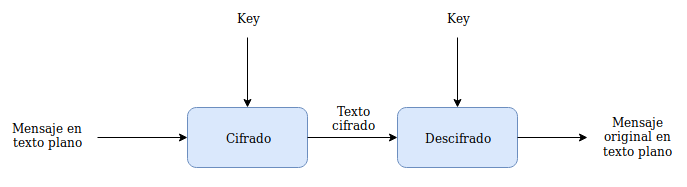
\includegraphics[width=14cm]{./imagenes/procesoCifrado.png}
				\caption{Proceso de cifrado y descifrado.}
			\end{center}
		\end{figure}
	
		%Estenografía
		\subsubsection{Estenografía.}
		
		La estenografía es una técnica en la criptografía, la cual tiene como objetivo lograr la confidencialidad sin ningún proceso de cifrado. Es una manera de esconder un mensaje secreto tal que la existencia del mensaje escondido sea imposible de detectar. Esto involucra esconder un mensaje oculto en algún tipo de archivo digital, el cual contiene bits redundantes donde poder esconder el mensaje, tal que altera los bits más insignificantes de cada byte del archivo digital con los bits del mensaje secreto.\\
		
		Como resultado de esto, la \textbf{NSA} y \textbf{FBI} declararon 2 formas que permiten al gobierno controlar la criptografía en Estados Unidos:
        \begin{enumerate}
            \item \textbf{Propuesta clave de depósito de garantía} (KEP): Esta propuesta requiere que el usuario se registre en su software de cifrado de llave con el gobierno.
            \item \textbf{Propuesta de Recuperacion de Clave} (KRP): Esta propuesta provee el permiso para el gobierno de tener acceso al ''\Gls{backdoor}'' para obtener la llave de acceso para descifrar el mensaje cifrado
        \end{enumerate}
		
		\subsection{Chaffing and Winnowing.}
		
		Chaffing and Winnowing es un nuevo esquema establecido por Rivest en 1998. Este esquema ofrece confidencialidad para el contenido de un mensaje sin involucrarse con cifrado ni estenografía, sin embargo, ofrece los cuatro objetivos principales de la Criptografía, los cuales son:
		\begin{enumerate}
			\item \textbf{Confidencialidad} Mantiene la información secreta para todos los usuarios excepto para los usuarios que estén autorizados para visualizarlos u obtenerlo.
			\item \textbf{Integridad de datos} Asegura que la información no haya sido alterada por medios no autorizados o desconocidos.
			\item \textbf{Autenticación} Confirma la identidad de una entidad.
			\item \textbf{No repudio} Previene la denegación de compromisos o acciones anteriores.
		\end{enumerate}

		El objetivo de \textbf{Chaffing and Winnowing} es asegurar que los adversarios no obtengan información del mensaje transmitido a lo largo de un canal de comunicación inseguro entre dos partes. El esquema de Rivest consiste en tres partes principales.
		\begin{enumerate}
		    \item \textbf{Autentificación} Es el proceso de descomponer el mensaje original en un paquete más pequeño y complementar cada paquete con un código de autentificación de mensaje (MAC).
		    \item \textbf{Chaffing} Es el proceso de agregar paquetes inválidos (Chaff packets).
		    \item \textbf{Winnowing} Es el proceso de remover paquetes Chaff para obtener el mensaje original en texto plano.
		\end{enumerate}
		
		El la figura 2, se muestra el paso "Chaffing", la cual muestra donde se agregan los paquetes inválidos (Chaff packets).
		\paragraph{}
		\textbf{Escenario 1:} Alice esta comunicando con Bob en un solo camino de comunicación sobre un canal inseguro y Charles (Proveedor de servicios de Internet) agrega los paquetes de Chaff.\\
		\begin{figure}[!htb]
			\begin{center}	                  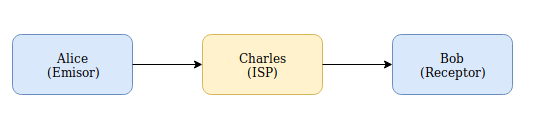
\includegraphics[width=14cm]{./imagenes/chaffProcess.png}
				\caption{Charles agrega los paquetes inválidos.}
			\end{center}
		\end{figure}
		
		En el escenario anterior Alice y Bob se están comunicando mutuamente por un canal de comunicación no seguro, en donde son enviados paquetes no cifrados. Alice y Bob comparten la llave de autenticación la cual será usada para el proceso de autenticación. Cuando Alice envía un mensaje a Bob, su mensaje es autenticado de su lado y es enviado a Charles antes de ser enviado a Bob. Charles agrega los paquetes chaff a la secuencia transmitida por Alice, al agregar los paquetes chaff, Charles provee confidencialidad para la comunicación entre Alice y Bob. Pero donde Charles no conoce la llave secreta compartida entre Alice y Bob. Por lo que el proceso de chaffing no necesita ningún conocimiento de la llave secreta de autenticación compartida.
		\paragraph{}
		\textbf{Escenario 2:} Alice se comunica con Bob en un camino de comunicación inseguro y en el cual Charles no agrega los paquetes chaff si no que multiplexa los flujos de las otras dos partes (David y Elaine). Este escenario es diferente al anterior, ya que se multiplexo el flujo de datos de Alice y Bob con el flujo de datos de David y Jane, y cuando el paquete llega a Bob el flujo de paquetes de David hacia Jane es el chaff de Bob y es descartado y vice versa para Jane.
		
		\begin{figure}[H]
			\begin{center}	                  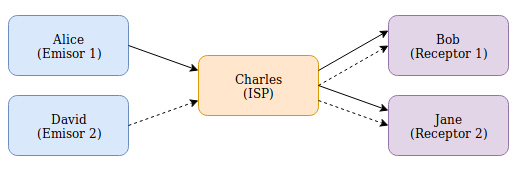
\includegraphics[width=14cm]{./imagenes/escenario2.png}
				\caption{Charles no agrega los paquetes pero multiplexa los flujos.}
			\end{center}
		\end{figure}
		
		\newpage
		\textbf{Escenario 3:} Alicia se comunica con Bob en un canal de comunicación inseguro y Alice no agrega los paquetes chaff. En este escenario, Alice desarrolla la autenticación de sus mensajes, por lo que Alice aplica chaffing para autenticar los mensajes y producir una secuencia de paquetes que serán transmitidos a Bob por la vía de Charles. Bob lleva a cabo el proceso de winnowing para recuperar el mensaje original.

		\subsubsection{¿Como funciona Chaffing and Winnowing?}
		
		El esquema de Chaffing and Winnowing deja que cada paquete conste de: un número de serie, contenido del paquete y el código de autenticación del mensaje.
		Cuando son enviados los paquetes, el mensaje con el texto plano se descompone en pequeños paquetes los cuales contienen datos y el tamaño del paquete original. Entonces, el emisor (Alice) usa el algoritmo de \textbf{código de autenticación de mensaje} (MAC) \Gls{HMACSHA14} para generar el valor MAC para ser agregado al paquete y el cual se basa en el número de serie, contenido del paquete y la llave autenticación. A continuación se muestra la salida del paquete después de la autenticación.
		
		\begin{figure}[H]
			\begin{center}	                  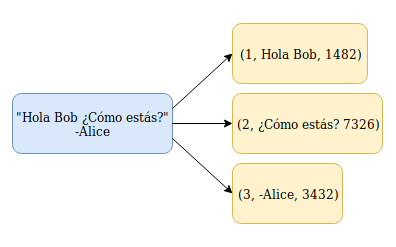
\includegraphics[width=8cm]{./imagenes/descomposicionChaffing.png}
				\caption{Secuencia de Chaffing después del proceso de autenticación.}
			\end{center}
		\end{figure}
		
		Esta secuencia de paquetes es enviada a Charles (ISP) para llevar a cabo el proceso de Chaffing. Charles agrega paquetes chaff a la secuencia de paquetes antes de ser enviados por medio del canal de comunicación y ser recibidos por Bob. Ahora, existen dos maneras donde Charles puede enviar la secuencia de chaff hacia Bob. La primera es enviando aleatoriamente mezclados los paquetes chaff para formar una secuencia y la otra manera es enviarlos de manera ordenada por el nÚmero de serie seguido del contenido del mensaje. En la siguiente figura se muestra cómo es el proceso de chaff en esta secuencia.
		
		\begin{figure}[H]
         \centering
          \subfloat[Primera manera]{
           \label{f:Primera manera}
            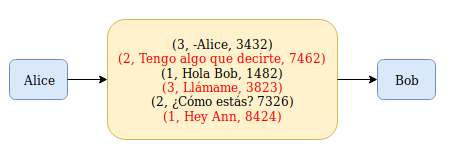
\includegraphics[width=0.5\textwidth]{./imagenes/firstway_Chaff.png}}
          \subfloat[Segunda manera]{
           \label{f:Segunda manera}
            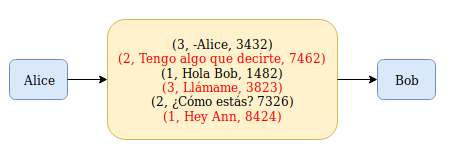
\includegraphics[width=0.5\textwidth]{./imagenes/firstway_Chaff.png}}
         \caption{Las dos maneras para el proceso de chaff pueden ser utilizadas. Los paquetes chaff son los mensajes de color rojo.}
         \label{f:Enfoques}
        \end{figure}
		
		Una vez que la secuencia de chaff llega a Bob, el último proceso es Winnowing. Bob determina la secuencia del mensaje que es válida del paquete chaff usando una función hash para el contenido de cada paquete y la llave de autenticación para re-calcular el MAC y compararlo contra el MAC del paquete recibido, si la comparación falla, el paquete chaff es descartado. 
		La siguiente imagen muestra el proceso completo de chaffing and winnowing.
		
		\begin{figure}[H]
			\begin{center}	                  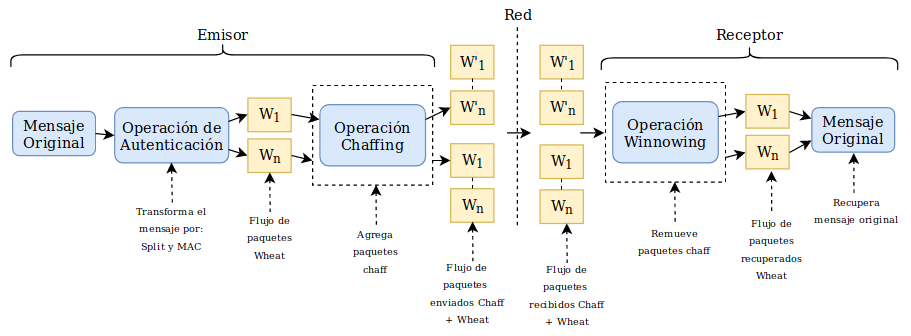
\includegraphics[width=14cm]{./imagenes/chaff_winn.png}
				\caption{Visión general del proceso Chaffing and Winnowing.}
			\end{center}
		\end{figure}
		
		\subsubsection{Propiedades de Chaffing and Winnowing}
		\begin{itemize}
		    \item La técnica de Chaffing y Winnowing no depende de la fuerza del esquema de cifrado para proporcionar confidencialidad debido al hecho de que es muy difícil distinguir el ''wheat'' de los paquetes chaff sin la clave secreta. Por lo tanto, la dificultad de distinguir el ''wheat'' del chaff proporciona confidencialidad al esquema.
		    \item La operación de Chaffing puede ser realizada por un tercero, ya que la clave secreta compartida no es necesaria en el proceso del mismo.
		    \item Los paquetes de Chaff no tienen que contener datos aleatorios, ya que uno podría usar un mensaje válido con una clave secreta diferente para hacer el paquete de Chaff. Cuando el receptor recibe esos paquetes de Chaff, se verán como paquetes de Chaff, ya que la clave que se usa para volver a calcular el Chaff es diferente de la que los hace.
		\end{itemize}
        
        \subsubsection{Enfoques alternativos para el esquema de Chaffing and Winnowing}
        
        Existes dos sugerencias que se pueden utilizar en este esquema. El primero es iniciar los paquetes ''Wheat'' que contienen un solo bit de datos y dejar los paquetes chaff con los bits complementarios. Ambos contienen un numero de serie y un valor hash del contenido del mensaje. Aplicando ésta sugerencia, se le será muy difícil y casi imposible al adversario identificar los paquetes ''wheat'' de los paquetes chaff. La siguiente figura demuestra como la secuencia chaff funcionaría si se le aplica ésta primer sugerencia.
        
        \begin{figure}[H]
			\begin{center}	          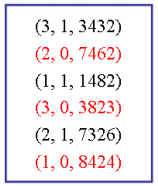
\includegraphics[width=3cm]{./imagenes/esquema1.png}
				\caption{Primer sugerencia, donde los paquetes chaff son de color rojo.}
			\end{center}
		\end{figure}
        
        Claramente, el esquema anterior es muy ineficiente cuando tratamos de enviar mensajes cortos o incluso mensajes largos. Esto puede comprobarse mediante un simple cálculo para mostrar la sobrecarga que se agrega con esta sugerencia.
        
        Supongamos que se utiliza una función hash cuyo valor de hash es de 64 bits de salida y cada paquete contiene un número de serie (1 bit de contenido de datos y el valor de hash del mensaje).
        
        Por lo tanto, tenemos 32 bits, (que es la representación máxima de un valor entero) para el número de serie, 1 bit para el contenido de datos y 64 bits para los valores hash. Entonces, cuando los paquetes ''wheat'' y el paquete chaff se están transmitiendo, tenemos lo siguiente:
        \begin{center}
        $32 + 1 + 64 = 97$
        \end{center}
        El cual es el número total de bits que se transmiten para un solo paquete ''wheat''
        \begin{center}
        $32 + 1 + 64 = 97$  
        \end{center}
        El cual es el número total de bits que se transmiten para un solo paquete chaff. Como resultado, este esquema requiere 194 bits para ser transmitido. Aunque esta técnica incremente la seguridad del esquema Chaffing and Winnowing debido a las características adicionales, éste enfoque no es muy eficiente. El valor hash puede ser otro valor como 128, 256, etc. dependiendo del bit de salida de la función hash.\\
        
        La segunda sugerencia es adoptar “All-or-Nothing and Package Transform, (AONT)”.
        Lo que permite muchos bits por paquete y reduce la sobrecarga adicional a cada paquete. 
        Cuando se transfiere un mensaje grande, ésta sugerencia es más eficiente. El detalle de la AONT se tratará en la siguiente sección.\\
        
        \textbf{All-or-Nothing and the Package Transform (AONT)}\\
        
        All-or-Nothing and the Package Transform es una variación dentro de la tecnica Chaffing and Winnowing, donde se mejora la eficiencia de su esquema original. AONT es la transformación de pre-procesamiento que permite a las partes enviar más datos (en términos de bit) por paquete en lugar de solo uno. Este pre-procesamiento es una transformación sin cifrado que toma el mensaje de texto sin formato y produce un mensaje empaquetado que luego se procesa de la manera normal de Chaffing and Winnowing. Las definiciones de la transformación AONT son las siguientes:
        
        \begin{enumerate}
            \item El algoritmo de transformación es \textbf{reversible}: Dado el bloque de mensaje transformado, el receptor puede obtener el mensaje de texto sin formato original.
            \item El algoritmo de transformación y su inverso son \textbf{computables} de manera eficiente: Lo que significa que es computacionalmente factible recrear el texto original dada la llave privada y recibir todos los paquetes con éxito.
            \item La transformación no es \textbf{computacionalmente factible}: Esto significa que si se ha recibido parte del paquete de la transmisión, cualquiera que esté intentando leer el mensaje no puede hacerlo ya que la transformación \textbf{AONT} requiere que se reciba todo el mensaje, de lo contrario no entrega nada.
            \item La transformación es una \textbf{técnica sin cifrado}: La técnica de pre-procesamiento no tiene llaves y no hay una llave secreta compartida involucrada en la operación. Cualquier persona que haya recibido todos los mensajes transformados del paquete puede recuperar el mensaje de texto original.
        \end{enumerate}
        
        \textbf{¿Cómo funciona AONT?}
        
        \paragraph{}
        Supongamos que el mensaje de entrada es el siguiente: $m_{1},m_{2},...,m_{n}$
        Seleccionamos una llave aleatoria $K'$ el cual se usará para la función del paquete de transformación.\\
        Se calcula la secuencia transformada ${m'}_{1}, {m'}_{2},...,{m'}_{s}$ para ${s'}=s+1$ como se muestra a continuación:\\
        Tenemos:
        \begin{center}
            $m_{i} \otimes E(K',i)$ for  $i=1,2,3,...,s$
        \end{center}
        También:
        \begin{center}
            $m'_{s'}=K' \otimes h_{1} \otimes h_{2} \otimes ... \otimes h_{s}$
        \end{center}
        
        Donde:
        \begin{center}
            $h_i=E(K_0,m'_i \otimes i)$ for $i=1,2,...,s$
        \end{center}
        
        Donde $K_0$ es una llave conocida pública fija.\\
        Para que el receptor en el otro extremo obtenga el $K_0$, el cual es la llave para el uso de \textbf{AONT}, el receptor realiza el siguiente cálculo:
        
        \begin{center}
            $K'=m'_s \otimes h_1 \otimes h_2 \otimes ... \otimes h_s$
        \end{center}
        \begin{center}
            $m_i=m'_i \otimes E(K',i)$ for $i=1,2,...,s$
        \end{center}
        
        \paragraph{}
        AONT toma el mensaje de texto sin formato de entrada y los transforma, luego crea un bloque para almacenar los mensajes transformados antes de pasar al proceso de autenticación. Después, se genera el paquete Chaff (la cantidad de paquetes Chaff no tiene que ser igual a los paquetes ''Wheat'').\\
        Esta técnica produce una menor sobrecarga que la sugerencia número 1. El AONT ofrece más confidencialidad al esquema de Chaffing and Winnowing, ya que el adversario debe recibir todo el bloque de mensajes de transformación e identificar correctamente todo el paquete ''wheat'' para obtener el mensaje de texto original. La siguiente figura muestra la
        descripción general de Chaffing y Winnowing si se agrega la función AONT.
        
        \begin{figure}[!htb]
			\begin{center}	          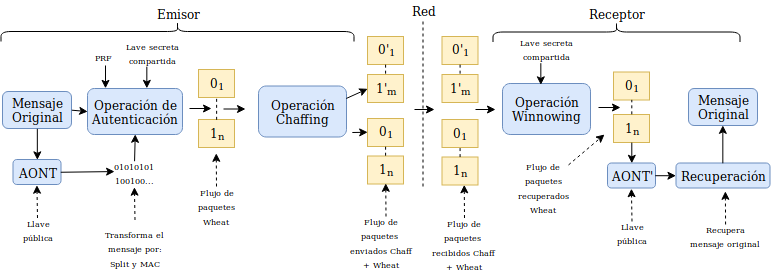
\includegraphics[width=14cm]{./imagenes/chaffVsCrypto.png}
				\caption{Proceso de Chaffing and Winnowing junto con AONT.}
			\end{center}
		\end{figure}
        
        \paragraph{}
        \textbf{¿Cómo AONT puede hacer la diferencia?}\\
        
        \begin{enumerate}
            \item Requiere menos ancho de banda al transferir paquetes, ya que se pueden transferir más bits en un paquete en lugar de un bit por paquete.
            \item Los paquetes Chaff son más fáciles de generar, ya que AONT transforma el mensaje de texto plano en bits aleatorios.
            \item La distinción entre Chaffing and Winnowing es más difícil: Si el adversario va a ejercer fuerza bruta en los paquetes, la tarea se ralentizará por el factor del número de bloque de mensajes. Dado que el bloque de mensaje de información adicional se mezcla aleatoriamente dentro de los flujos de paquetes de Chaffing and Winnowing, sin saber que es muy difícil que el bloque adicional proporcione la posibilidad de elegir el bloque de mensaje correcto de los paquetes para obtener el texto plano original.
        \end{enumerate}
        
        \subsubsection{Comparando Chaffing and Winnowing contra Cifrado y Estenografía}
        
        En esta sección explicaremos porque Chaffing and Winnowing no puede ser clasificado como una técnica de cifrado o Estenografía.\\
        
        \textbf{Chafing and Winnowing vs Cifrado}\\
        
        Nosotros podríamos clasificar Chaffing and Winnowing como un método de cifrado, pero volvamos a recordar el principio de un Cifrado.
        El principal objetivo de un cifrado es ocultar el mensaje en texto plano de tal manera que oculta su contenido con el uso de una clave de cifrado para el texto cifrado.
        Por otro lado, en el esquema original de Chaffing and Winnowing, una llave compartida es usada con el fin de autenticar la validación de los paquetes ya sea del emisor o del receptor. Además, Chaffing and Winnowing no hace uso de ninguna técnica de cifrado para ocultar el contenido de un mensaje y que nadie pueda ver dicho mensaje, solo aquellos con la llave correspondiente pueden determinar que paquetes contienen la información valida. A continuación, se muestra como se puede ver el esquema Chaffing and Winnowing como una técnica de cifrado. 
        
        \begin{figure}[H]
			\begin{center}	                  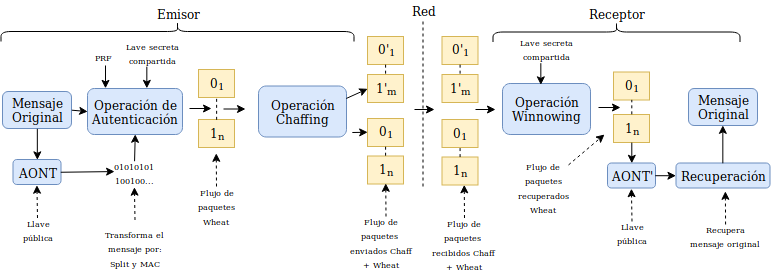
\includegraphics[width=14cm]{./imagenes/chaffVsCrypto.png}
				\caption{Visualizando el método Chaffing and Winnowing cómo un esquema de cifrado.}
			\end{center}
		\end{figure}
        
        Chaffing y Winnowing pueden verse como \textbf{un tipo especial de esquema de cifrado simétrico}, ya que la operación \textbf{chaffing} es similar al ''proceso de cifrado''. En la operación de chaffing, el texto cifrado se crea para producir un paquete ''wheat'' no válido que se envía al receptor. Luego, el receptor realiza el ''proceso de descifrado'', que implica descartar el paquete de desperdicios y recuperar el mensaje original. Ambas operaciones operan bajo una llave secreta común que se usa para derivar el valor MAC.\\
        
        Pero la diferencia es, \textit{Chaffing y Winnowing} dos partes no buscan lograr la confidencialidad. El emisor comparte una clave secreta con el receptor para que el receptor pueda usar la clave secreta para autenticarse (si se afirma que el mensaje recibido proviene del remitente deseado). Pero la ganancia de confidencialidad proviene de la dificultad de distinguir el paquete Chaff del paquete ''Wheat''. Mientras que en el cifrado, la clave se utiliza para lograr la confidencialidad mediante la creación de texto cifrado que oculta el contenido del mensaje de personas.
        
        Con Chaffing y Winnowing con el esquema AONT, el esquema en sí es muy parecido al cifrado, excepto que la clave que se usa en la transformación AONT se elige aleatoriamente cada vez en lugar de fijarla. Además, el último bloque de mensajes es exclusivo o de la clave y todo el hash del bloque de mensajes está allí para garantizar que cualquier modificación en el bloque de mensajes cambiará la clave $K'$ calculado por el receptor. Por lo tanto, el último bloque de mensajes ${m'}_s'$ está allí solo con el propósito de autenticación. Por lo tanto, Chaffing y Winnowing con el esquema AONT no pueden ser clasificados bajo cifrado.\\
        
        \textbf{Chaffing and Winnowing vs Estenografía}\\
        
        Para algunas personas, Chaffing and Winnowing puede ser clasificado como una técnica estenográfica. Sin embargo, el objetivo principal de la estenografía es el de ocultar el mensaje original dentro de otro tipo de mensaje, por lo tanto, nadie aparte del emisor y el receptor sabrá que hay un mensaje oculto. Contrario a Chaffing and Winnowing, en donde cualquiera puede ver el contenido del mensaje, ya que este método no trata de esconderlo de los posibles atacantes.\\
        Otra diferencia es que en estenografía el emisor tiene que ocultar el mensaje el mismo, mientras que en Chaffing and Winnowing no necesariamente es así, ya que una "tercera parte" puede hacerlo.\\
        Por lo tanto, Chaffing and Winnowing no puede ser considerado como estenografía.\\
        
        Para nuestro proyecto usaremos \textit{Chaffing and Winnowing}, para proponer un nuevo método de autentificación para servicios web. \\
        
        
		
	    %%%%%%%%%%% ALGO DE SEPARACIÓN
		
		Primero, empezaremos por tener un mejor panorama acerca de los diferentes métodos de autentificación. En el cuadro No.1, se comparan algunos de éstos diferentes métodos basándose en la simplicidad de su aplicación para el usuario \cite{ComparisonAuthenticationMethodsResources} Donde: 1 – Bajo desempeño, 2 - Medio desempeño y 3 – Alto desempeño.
		
		\begin{table}[H]
			\centering
			\resizebox{13cm}{!} {
				\begin{tabular}{l|l|l|l|l|l|l|l|}
					\cline{2-8}
					& Recordar & \begin{tabular}[c]{@{}l@{}}Otros\\ dispositivos\end{tabular} & Acciones & Facilidad & Tiempo & Errores & Recuperación \\ \hline
					\multicolumn{1}{|l|}{Contraseñas}                                                      & 1        & 3                                                            & 2        & 3         & 3      & 2       & 3            \\ \hline
					\multicolumn{1}{|l|}{Otros recursos}                                                   & 2        & 3                                                            & 3        & 3         & 3      & 3       & 2            \\ \hline
					\multicolumn{1}{|l|}{\begin{tabular}[c]{@{}l@{}}Contraseñas \\ gráficas\end{tabular}}  & 1        & 1                                                            & 2        & 3         & 3      & 2       & 3            \\ \hline
					\multicolumn{1}{|l|}{\begin{tabular}[c]{@{}l@{}}Contraseñas \\ dinámicas\end{tabular}} & 1        & 3                                                            & 2        & 2         & 3      & 2       & 2            \\ \hline
					\multicolumn{1}{|l|}{Tokens}                                                           & 3        & 1                                                            & 1        & 2         & 2      & 3       & 1            \\ \hline
					\multicolumn{1}{|l|}{Multivariación}                                                   & 1        & 1                                                            & 1        & 3         & 2      & 2       & 1            \\ \hline
					\multicolumn{1}{|l|}{Cryptografía}                                                     & 3        & 1                                                            & 1        & 1         & 1      & 2       & 1            \\ \hline
					\multicolumn{1}{|l|}{Biométricos}                                                      & 3        & 3                                                            & 2        & 3         & 2      & 2       & 1            \\ \hline
				\end{tabular}
			}
			\caption{Comparación de la aplicación en los distintos métodos de autentificación}
		\end{table}
		La tabla anterior concentra las siguientes características:
		
		\begin{itemize}
			\item Recordar: Hace referencia a que tan complicado es que un usuario se acuerde de los datos necesarios para la autentificación. 
			\item Otros dispositivos: El usuario usa una entidad externa para facilitar su autentificación.
			\item Acciones: Hace referencia a que tantas acciones adicionales se deben de realizar para autentificarse.
			\item Facilidad: Simplicidad de tecnología.
			\item Tiempo: Cantidad de recursos temporales que consume el método de autentificación.
			\item Errores: Posibles errores durante la autentificación. 
			\item Recuperación: Denota la dificultad de recuperar la clave de acceso en caso de pérdida.
		\end{itemize}
		
		En el cuadro No.2 se muestra una tabla comparativa del nivel de seguridad en los distintos métodos de autentificación, donde 1 - baja seguridad, 2 – media seguridad y 3 – alta seguridad.
		
		\begin{table}[H]
			\centering
			\resizebox{10cm}{!} {
				\begin{tabular}{l|l|l|l|l|}
					\cline{2-5}
					& \begin{tabular}[c]{@{}l@{}}Ataque por\\ fuerza bruta\end{tabular} & Observación & \begin{tabular}[c]{@{}l@{}}Hackeo\\ indirecto\end{tabular} & Phishing \\ \hline
					\multicolumn{1}{|l|}{Contraseñas}                                                      & 1                                                                 & 1           & 1                                                          & 1        \\ \hline
					\multicolumn{1}{|l|}{Otros recursos}                                                   & 2                                                                 & 2           & 3                                                          & 3        \\ \hline
					\multicolumn{1}{|l|}{\begin{tabular}[c]{@{}l@{}}Contraseñas \\ gráficas\end{tabular}}  & 1                                                                 & 1           & 2                                                          & 2        \\ \hline
					\multicolumn{1}{|l|}{\begin{tabular}[c]{@{}l@{}}Contraseñas \\ dinamicas\end{tabular}} & 2                                                                 & 3           & 2                                                          & 2        \\ \hline
					\multicolumn{1}{|l|}{Tokens}                                                           & 3                                                                 & 3           & 3                                                          & 3        \\ \hline
					\multicolumn{1}{|l|}{Multivariación}                                                   & 1                                                                 & 1           & 3                                                          & 3        \\ \hline
					\multicolumn{1}{|l|}{Cryptografía}                                                     & 3                                                                 & 3           & 3                                                          & 3        \\ \hline
					\multicolumn{1}{|l|}{Biométricos}                                                      & 3                                                                 & 3           & 1                                                          & 1        \\ \hline
				\end{tabular}
			}
			\caption{Comparación de la seguridad en los distintos métodos de autentificación}
		\end{table}
		La tabla se enfoca principalmente en los siguientes problemas de seguridad: 
		
		\begin{itemize}
			\item Ataque por fuerza bruta: Se descifra el método de autentificación con una gran cantidad de intentos, usualmente generados por un programa.
			\item Observación: Cuando se intenta ver directamente los datos necesarios para la autentificación desde una distancia cercana hasta incluso usando binoculares, cámaras o algún otro dispositivo.
			\item Hackeo indirecto: El usuario confía sus datos del método de autentificación a terceros quienes pueden ser atacados. 
			\item Phishing: Hace referencia a programas que se hacen pasar por entidades confiables para interceptar los datos que desean.
		\end{itemize}
		
		\paragraph{Clasificación de ataques web}
		\begin{itemize}
		\item Ataques \acrshort{url} de tipo semántico\\
		Este tipo de ataques involucran a un usuario modificando la \acrshort{url} a modo de descubrir acciones a realizar que originalmente no están planeadas para ser manejadas correctamente por el servidor. La implementación de cualquier formulario debe contemplar validaciones necesarias para evitar el esas acciones y se deben realizar adecuaciones de acuerdo a nuestras entradas.
		\item Ataques de Cross-Site Scripting \\
		Cross-Site Scripting (XSS) es un tipo de vulnerabilidad de seguridad informática típicamente encontrada en aplicaciones web que permiten la inyección de código por usuarios maliciosos en páginas web. Los atacantes se valen de código \acrshort{html} y de scripts ejecutados en el cliente. 
		
		\begin{table}[H]
			\centering
		    \resizebox{14cm}{!} {
                \begin{tabular}{|c|c|c|}
                \hline
                Tipo   & Nombre                           & Descripción                                                                                                                                                                                                                                                                                                   \\ \hline
                Tipo 0 & Ataque basado en el DOM o local  & \begin{tabular}[c]{@{}c@{}}Si un código de JavaScript accede a una URL como \\ un parámetro de una petición al servidor y utiliza un \\ parametro de una petición al servidor y utiliza esta \\ información para escribir HTML en la misma página \\ sin ser codificada empleando entidades \acrshort{html}\end{tabular} \\ \hline
                Tipo 1 & Ataque no persistente o relajado & \begin{tabular}[c]{@{}c@{}}Si los datos no válidos por el usuario son incluidos en \\ la página resultante sin codificación \acrshort{html}, se le permite \\ al cliente inyectar código en la página dinámica\end{tabular} \\ \hline
                Tipo 2 & Ataque persistente o almacenado  & \begin{tabular}[c]{@{}c@{}}La información proporcionada por el usuario \\ es almacenada en la base de datos, en el sistema\\ de archivos o algún otro lugar; después es mostrada\\ a otros usuarios que visiten la página\end{tabular}                                                                        \\ \hline
                \end{tabular}
            }
        \end{table}
		
		\item Ataques de Cross-Site Request Forgery \\
		Este tipo de ataque permite al atacante enviar peticiones \acrshort{http} a voluntad desde la máquina de la víctima. Es difícil determinar cuándo una petición \acrshort{html} se ha originado por un ataque de este tipo.

        Cuando un atacante conoce el formato que debe tener una URL para lograr la ejecución de una acción en el sistema, ha logrado encontrar la posibilidad de explotar este tipo de ataques. Lo único que necesita el atacante es simplemente hacer que una víctima visite la URL.
		
		\item Peticiones \acrshort{http} falsificadas\\
		Un ataque más sofisticado es enviar peticiones falsas empleando herramientas especiales para este propósito.

        Para ello, se emplean herramientas de línea de comandos o plugins agregados a los navegadores, con estos se pone a la escucha de los servicios web que típicamente se conectan a través del puerto 80.
		\end{itemize}
		
		\paragraph{Seguridad de las aplicaciones relacionado a la base de datos} 
		\begin{itemize}
		    \item Exposición de Credenciales de Acceso \\
		    Uno de los asuntos principales a ser cuidados cuando se utiliza una base de datos es el almacenamiento de las credenciales de acceso a ella.

            Los datos de usuario y contraseña son considerados sensibles, por lo que deben tener garantizada una atención especial. En archivos de configuración es común encontrar estos datos los cuales se encuentran como texto en claro.
            La intercepción o acceso no autorizado de esta información podría comprometer los servidores de bases de datos o  gestores de contenidos en donde estén alojados. 
            
            \item Exposición de datos \\
            Una de las preocupaciones más comunes relacionadas con las bases de datos es la exposición de datos sensibles. Al almacenar números de tarjetas de crédito, por ejemplo, es preferible asegurarse que los datos almacenados en la base de datos se encuentran seguros e inaccesibles incluso para los administradores de la base.

            Para asegurar que no se almacenan datos como texto en claro en la base de datos, se pueden realizar procedimientos de hash a las cadenas almacenadas para que no sea entendible la información a simple vista. Se debe considerar el costo de esta implementación ya que habría que obtener el hash al insertarlo y al extraerlo realizar la operación inversa, lo que conllevaría a que la aplicación tarde un poco más en responder.
            
		\end{itemize}
		
		\paragraph{Páginas privadas y los sistemas de autenticación}
		\begin{itemize}
		    \item La autenticación consiste en verificar la identidad de un usuario. Comúnmente el procedimiento involucra un nombre de usuario y una contraseña a revisar. Muchas aplicaciones tienen recursos que son accesibles sólo para los usuarios autenticados, así como recursos totalmente públicos.
		    
		    \item Ataques de fuerza bruta \\
		    Este tipo de ataque es un método de ensayo y error utilizado para obtener información de una contraseña, clave o número de identificación personal, entre otros. Funciona mediante la generación de un gran número de intentos consecutivos para el valor de los datos deseados. Un ataque de este tipo agota todas las posibilidades sin preocuparse por cuales opciones tienen mayor probabilidad de funcionar.
            En los términos del control de acceso, generalmente encontramos al atacante intentando ingresar mediante un gran número de pruebas. En algunos casos el atacante puede conocer nombres de usuario válidos y la contraseña es la única parte que se trata de adivinar.
            
            \item Espionaje de contraseñas (Password Sniffing)\\
            En la actualidad debido a la información que se transmite en la web se recomienda establecer el uso del protocolo \acrshort{http}S para poder cifrar el canal de comunicación por el que se se envía la información. (OWASP, 2016)
            
            \item Cookies o variables de sesión persistentes\\
            Cuando un usuario permanece en el estado de registrado después de un tiempo no razonable, se tiene un problema de registros persistentes.
            Este tipo de problemas disminuyen la seguridad del mecanismo de autenticación. \\
            Generalmente son causados por una cookie persistente, un ticket enviado al usuario o alguna variable de sesión establecida que no se considera como expirado jamás o que no cambia en cada nuevo registro establecido por el usuario.
            Las cookies permanentes y variables de sesión ayudan a los sitios web a recordar la información de los usuarios y sus ajustes cuando visitan la páginas más adelante. Esto conlleva un acceso más rápido y sencillo ya que, el usuario no tiene que iniciar sesión de nuevo.
            
		\end{itemize}
		
	\newpage
	
	\section{\textcolor{azulescom}{Análisis.}}
	    
	    %   %   %   %   %   %   %   %   %   
		%		                        %
		%   ANÁLISIS DE PROTOTIPO I.    %
		%                               %
	    %   %   %   %   %   %   %   %   %
	    
		\subsection{Prototipo I.}
			\subsubsection{Descripción.}
				En este prototipo se busca la creación de una extensión de Google Chrome que pueda interceptar una petición \acrshort{http} hecha por el mismo navegador. Mientras la extensión se encuentre habilitada, será capaz de poder recibir las peticiones realizadas por el navegador y evitar que ésta sea mandada al servidor. Además mostrará en otra pestaña del navegador información sobre la petición interceptada. \\\\
				El propósito de realizar este prototipo es familiarizarse con el manejo de extensiones en el navegador Google Chrome; como es que podemos obtener la información que necesitamos para que posteriormente modifiquemos esta petición y la enviemos al servidor. 
			
			\subsubsection{Herramientas a usar.}
				\paragraph{Software. \\}
				Para el desarrollo de software de este prototipo, es necesario hacer mención de algunas de las siguientes herramientas, para tener una idea clara sobre qué herramientas estamos utilizando y porque es que las estamos utilizando:
				
				\paragraph{HTML5. \\}
				\acrlong{html} comenzó mucho tiempo atrás con una simple versión propuesta para crear la estructura básica de páginas web, organizar su contenido y compartir información, todo esto tenía la intención de comunicar información por medio de texto. El limitado objetivo de \acrshort{html} motivó a varias compañías a desarrollar nuevos lenguajes y programas para agregar características a la web nunca antes implementadas. \\\\
				Dos de las opciones propuestas fueron Java y \Gls{Flash}; ambas fueron muy aceptadas y consideradas como el objetivo de la internet, sin embargo, con el crecimiento exponencial del internet, éste dejó de ser únicamente para los aficionados de los computadores y pasó a ser usado como un campo estratégico para los negocios y para la interacción social, ciertas limitaciones presentes en ambas tecnologías probaron ser una sentencia de muerte. Esta falta de integración resultó ser crítica y preparó el camino para la evaluación de un lenguaje del cual hablaremos un poco más a detalle después: JavaScript. Sin embargo, pese a su gran impacto, el mercado no terminó de adoptarlo plenamente y rápidamente su popularidad fue declinando, y el mercado terminó enfocando su atención a Flash. No fue hasta que los navegadores mejoraron su intérprete para JavaScript y la gente se empezaba a dar cuenta de las limitaciones que ofrecía Flash, que JavaScript fue implementado y comenzó a innovar la forma en la que se programaba la web. Al cabo de unos años, JavaScript, \acrshort{html} y \acrshort{css} eran considerados como la más perfecta combinación para evolucionar la Web. \\\\
				HTML5 es una mejora de esta combinación, lo que unió todos estos elementos. HTML5 propone estándares para cada aspecto de la Web y también un propósito claro para cada una de las tecnologías involucradas. A partir de esto, \acrshort{html} provee los elementos estructurales, CSS se concentra en como volver esta estructura utilizable y atractiva a la vista, y JavaScript tiene todo lo necesario para brindar dinamismo y construir aplicaciones web completamente funcionales. Cabe mencionar que HTML5 funciona diferente dependiendo del navegador y la versión en la que se esté trabajando, algunos soportan más carcterísticas o diferentes funcionalidades que otros.
				\cite{refElGranLibro}%Pag 19 pdf
				
				\paragraph{Materialize. \\}
				
				
				
				\paragraph {JavaScript. \\}
				JavaScript es considerado como el lenguaje de programación de \acrshort{html} y de la web. Es un lenguaje de programación fácil de usar y muy versátil para el ámbito de la comunicación en redes. Los programas, llamados "scripts", se ejecutan en el navegador (Mozilla, Google Chrome, Internet Explorer, etc.) normalmente consisten en unas funciones que son llamadas desde el propio \acrshort{html} cuando algún evento sucede.\\\\
				Su primera aproximación a un uso real, fue en mayor parte para "dar vida a una página web", como dar animaciones a un botón, interacciones en tiempo real, entre otras más. 
				JavaScript fue desarrollado por \Gls{NetScape}, a partir del lenguaje Java, que en ese momento tenía mucho auge y popularidad, y su principal diferencia es que JavaScript sólo "funciona" dentro de una página \acrshort{html}.\\
				JavaScript fue declarado como estándar del European Computer Manufacturers Association (ECMA) en 1997, y poco después, también fue estandarizado por ISO.\cite{refJavaScript} \\\\ 
				JavaScript es un lenguaje interpretado, usado mayormente como complemento de ciertos objetivos específicos, sin embargo, uno de las innovaciones que ayudó a JavaScript fue el desarrollo de nuevos motores de interpretación, creados para acelerar el procesamiento del código. La clave de los motores más exitosos fue transformar el código de Javascript en código máquina para obtener una velocidad de ejecución mejor que antes. Esto a la vez permitió superar viejas limitaciones de rendimiento y confirmar el lenguaje JavaScript como la mejor opción para la Web.\\\\
				Para aprovechar esta prometedora plataforma de trabajo ofrecida por los nuevos navegadores, JavaScript fue expandido en cuestión de portabilidad e integración, a la vez, interfaces de programación de aplicaciones (APIs) fueron incorporando por defecto con cada navegador para asistir a JavaScript en funciones elementales. El objetivo de esto, fue principalmente hacer disponible poderosas funciones a través de técnicas de programación sencillas y estándares, expandiendo el alcance del lenguaje y facilitando la creación de programas útiles para la Web.\cite{refElGranLibro}
				
				
				\paragraph{Hardware. \\}
				En el ámbito del hardware, utilizaremos los equipos de cómputo con los cuales contamos actualmente los integrantes de este equipo, los cuales se especificarán a continuación: 
				
				\begin{table}[H]
					\begin{tabular}{|p{3.5cm}||p{10cm}|}
						\rowcolor{guindapoli}
						\multicolumn{2}{|c|}{\textbf{\textcolor{white}{Equipo de hardware utilizado.}}}\\
						\hline
						\rowcolor{white}Nombre & Morales González Diego Arturo\\
						\hline
						\rowcolor{azulclaro}Marca & Asus\\
						\hline
						\rowcolor{white}Modelo & X550VC\\
						\hline
						\rowcolor{azulclaro}Procesador & Intel Core i5\\
						\hline
						\rowcolor{white}Tarjeta de video & NVidia GForce 720\\
						\hline
						\rowcolor{azulclaro}Memoria RAM & 12 GB\\
						\hline
						\rowcolor{white}Disco duro & 1TB\\
					\end{tabular}
				\end{table}
				
				\begin{table}[H]
					\begin{tabular}{|p{3.5cm}||p{10cm}|}
						\rowcolor{guindapoli}
						\multicolumn{2}{|c|}{\textbf{\textcolor{white}{Equipo de hardware utilizado.}}}\\
						\hline
						\rowcolor{white}Nombre & Carrillo Fernández Gerardo\\
						\hline
						\rowcolor{azulclaro}Marca & HP\\
						\hline
						\rowcolor{white}Modelo & Pavilion g4\\
						\hline
						\rowcolor{azulclaro}Procesador & Intel Core i3\\
						\hline
						\rowcolor{white}Tarjeta de video & Intel Sandybridge Mobile\\
						\hline
						\rowcolor{azulclaro}Memoria RAM & 6 GB\\
						\hline
						\rowcolor{white}Disco duro & 500GB\\
					\end{tabular}
				\end{table}
			\newpage
			
			\subsubsection{Estudio de requerimientos.}
				\paragraph{Requerimientos Funcionales.\\ \\}
				{\setlength{\parindent}{12pt}
				\textbf{PI\_RF1. Interceptar petición \acrshort{http}.} La extensión deberá interceptar la petición \acrshort{http} del navegador, en cuanto el usuario realice alguna a través del navegador.\\

				\textbf{PI\_RF2. Deshabilitar extensión.} El usuario podrá deshabilitar la extensión, para que ésta no vigile su actividad en el navegador.\\
				
				\textbf{PI\_RF3. Habilitar extensión.} El usuario podrá habilitar la extensión, para que ésta vigile constantemente cuando éste realice una petición \acrshort{http}.\\
				
				\textbf{PI\_RF4. Validar petición.} La extensión deberá analizar la petición previamente recibida, y validar si ésta es HTTP(S) o no.\\
		        
				\textbf{PI\_RF5. Mostrar petición.} La extensión deberá mostrar en otra pestaña del navegador, la información de la petición que se haya realizado.\\
				
				\textbf{PI\_RF6. Evitar salida de petición.} La extensión deberá evitar que la petición salga red, deteniendola hasta cuando sea necesario. 
		        }
				
				\paragraph{Requerimientos no Funcionales.\\ \\}
				{\setlength{\parindent}{12pt}
				
				\textbf{PI\_RNF1. Plataforma de implementación.} La extensión será implementada en el navegador Google Chrome.\\
				
				\textbf{PI\_RNF2. Versión del navegador} La extensión funcionará a partir de la versión 65.0.3325.181.\\
				
				\textbf{PI\_RNF3. Tecnologías para la interfaz de usuario} Para el sistema se hará uso de \acrshort{html}, JavaScript, \acrshort{css}, JSON.\\
				
				\textbf{PI\_RNF4. Permitir ejecución de JavaScript en Google Chrome.} Para el correcto funcionamiento de la extensión, es necesario que se permita la ejecución de javascript en el navegador Google Chrome.
				}
			
			\subsubsection{Reglas del negocio.}
				{\setlength{\parindent}{12pt}
				\label{PI_RN1}
				\textbf{PI\_RN1. Confidencialidad de la actividad web.} En cuando el usuario lo indique por medio de la \acrlong{iu}, la extensión deberá dejar de vigilar la actividad que el usuario realice en el navegador. De igual forma, si el usuario indicara que permite que la extensión vigile la actividad web, ésta así lo hará.\\
				}\newpage
				
        %   %   %   %   %   %   %   %   %   
		%		                        %
		%   ANÁLISIS DE PROTOTIPO II    %
		%                               %
	    %   %   %   %   %   %   %   %   %
		
		\subsection{Prototipo II.}
		    \subsubsection{Descripción.}
		    En este prototipo se busca que la extensión de Google Chrome pueda modificar la petición HTTP previamente interceptada. La modificación se hará sólo mientras la extensión esté habilitada, y tiene como objetivo inyectar el código autentificador en el encabezado del protocolo. Una vez que dicho código es inyectado, la extensión deberá liberar la petición para que salga a red y llegue al servidor del servicio web correspondiente.\\
		    
		    El propósito de este prototipo es utilizar la técnica de \textit{Chaffing and winnowing} en este método de autentificación propuesto, para evitarle al usuario la tediosa tarea de ingresar sus credenciales y brindarle la seguridad necesaria al iniciar de sesión.
		    
		    \subsubsection{Herramientas a usar.}
		    \subsubsection{Estudio de requerimientos.}
		    \subsubsection{Reglas del negocio.}
	\newpage
	
	    %   %   %   %   %   %   %   %   %   
		%		                        %
		%           DESARROLLO          %
		%                               %
	    %   %   %   %   %   %   %   %   %
	
	\section{\textcolor{azulescom}{Desarrollo.}}
		\subsection{Prototipo I.}
			\subsubsection{Diagrama de casos de uso.}

				Diagrama de casos de uso general para el prototipo I.
				\begin{figure}[htb]
					\begin{center}
			    	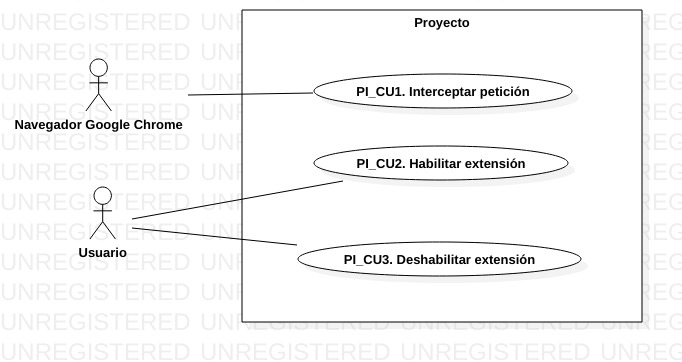
\includegraphics[width=14cm]{./imagenes/UCD_P1.jpg}
						\caption{Diagrama de casos de uso del Prototipo I.}
					\end{center}
				\end{figure}\newpage	
					
			\subsubsection{Descripción de casos de uso.}
			
				%%DESCRIPCIÓN PI_CU1
				\begin{table}[H]
				\begin{tabular}{ |p{3.5cm}||p{9.5cm}|}
					\hline
					\rowcolor{guindapoli}
					\multicolumn{2}{|c|}{\textbf{\textcolor{white}{Caso de uso: PI\_CU1. Interceptar petición.}}}\\
					\hline
					\rowcolor{azulfuerte}Concepto & Descripción\\
					\hline
					\cellcolor{azulclaro}Actor & 
					Navegador de Google Chrome.\\ 
					\hline
					\cellcolor{azulclaro}Propósito &
					Este caso de uso permite a la extensión interceptar una petición \acrshort{http}, realizada por el navegador Google Chrome por medio de algún agente (sistema o usuario) externo a éste.\\
					\hline
					\cellcolor{azulclaro}Entradas &
					Petición \acrshort{http} realizada por el navegador.\\
					\hline
					\cellcolor{azulclaro}Salidas &
					Petición \acrshort{http} cachada.\\
					\hline
					\cellcolor{azulclaro}Pre-condiciones&
					Algún agente externo (Sistema o usuario) ha ordenado al navegador mandar una petición \acrshort{http}.\\
					\hline
					\cellcolor{azulclaro}Post-condiciones&
					La extensión, deberá de interceptar la petición para poder modificarla.\\
					\hline
					\cellcolor{azulclaro}Reglas del negocio&
					-\\
					\hline
					\cellcolor{azulclaro}Errores &
					La petición no se pudo interceptar. \newline La petición no es tipo \acrshort{http}.\\					
					\hline
				\end{tabular}
				\caption[DCU: PI\_CU1]{Descripción CU: PI\_CU1}
				\end{table}
				
				\paragraph{... Trayectoria Principal ...}
				\begin{enumerate}
					\item \textbf{\textit{El Usuario}} o \textbf{\textit{El Sistema Externo}} realiza una petición \acrshort{http} en el navegador Google Chrome.\\
					\item \textbf{\textit{La Extensión}} intercepta la petición antes de que salga a red.\\
					\item \textbf{\textit{La Extensión}} puede modificar el contenido de la petición. \\
				\end{enumerate}
				\paragraph{... Fin de la Trayectoria Principal ...}
				
				\paragraph{... Trayectoria Alternativa 1 ...}
				\begin{enumerate}
					\item \textbf{\textit{El Usuario}} o \textbf{\textit{El Sistema Externo}} no realiza una petición \acrshort{http} en el navegador Google Chrome.\\
					\item \textbf{\textit{La Extensión}} ignora la petición.					
				\end{enumerate}
				\paragraph{... Fin de la Trayectoria Alternativa 1 ...}
				
				\paragraph{... Trayectoria Alternativa 2 ...}
				\begin{enumerate}
					\item \textbf{\textit{El Usuario}} o \textbf{\textit{El Sistema Externo}} realiza una petición \acrshort{http} en el navegador Google Chrome.\\
					\item \textbf{\textit{La Extensión}} no puede interceptar la petición antes de que salga a red.\\
					\item \textbf{\textit{La Extensión}} notifica que hubo un error al intentar interceptar la petición. 
				\end{enumerate}
				\paragraph{... Fin de la Trayectoria Alternativa 2 ...}
				
				\newpage
				%%DESCRIPCIÓN PI_CU2
				\begin{table}[H]
				\begin{center}
				\begin{tabular}{ |p{3.5cm}||p{9.5cm}|}
					\hline
					\rowcolor{guindapoli}
					\multicolumn{2}{|c|}{\textbf{\textcolor{white}{Caso de uso: PI\_CU2. Habilitar extensión.}}}\\
					\hline
					\rowcolor{azulfuerte}Concepto & Descripción\\
					\hline
					\cellcolor{azulclaro}Actor & 
					Usuario.\\ 
					\hline
					\cellcolor{azulclaro}Propósito &
					Este caso de uso, permite al usuario habilitar a la extensión, para que ésta sea capaz de ver todas las peticiones que realiza el navegador.\\
					\hline
					\cellcolor{azulclaro}Entradas &
					Indicación de habilitar extensión, mediante interfaz de usuario.\\
					\hline
					\cellcolor{azulclaro}Salidas &
					Ninguna.\\
					\hline
					\cellcolor{azulclaro}Pre-condiciones&
					El usuario debe de haber instalado la extensión en Google Chrome y haber permitido su ejecución.\\
					\hline
					\cellcolor{azulclaro}Post-condiciones&
					La extensión verá todas las peticiones que realice el navegador.\\
					\hline
					\cellcolor{azulclaro}Reglas del negocio&
					\hyperref[PI_RN1]{PI\_RN1.}\\
					\hline
					\cellcolor{azulclaro}Errores &
					No se puede iniciar la vigilancia de la extensión.\\
					
					\hline
				\end{tabular}
				\caption[DCU: PI\_CU2]{Descripción CU: PI\_CU2}
				\end{center}
				\end{table}
				
				\paragraph{... Trayectoria Principal ...}
				\begin{enumerate}
					\item \textbf{\textit{El usuario}} da click en el ícono de la extensión \textbf{insert icon}.
					\item \textbf{\textit{El usuario}} da click en el botón \textbf{insert button} "Habilitar extensión".
					\item \textbf{\textit{La extensión}} empieza a vigilar las peticiones que se realicen a través del navegador.
				\end{enumerate}
				\paragraph{... Fin de la Trayectoria Principal ...}
				
				\paragraph{... Trayectoria Alternativa 1 ...}
				\begin{enumerate}
					\item \textbf{\textit{El usuario}} da click en el ícono de la extensión \textbf{insert icon}.
					\item \textbf{\textit{El usuario}} da click en el botón \textbf{insert button} "Deshabilitar extensión".
					\item \textbf{\textit{La extensión}} muestra mensaje de error "La extensión ya está deshabilitada".
				\end{enumerate}
				\paragraph{... Fin de la Trayectoria Alternativa 1 ...}
				
				\paragraph{... Trayectoria Alternativa 2 ...}
				\begin{enumerate}
					\item \textbf{\textit{El usuario}} no encuentra el ícono de la extensión \textbf{insert icon}.
				\end{enumerate}
				\paragraph{... Fin de la Trayectoria Alternativa 2 ...}
				
				\newpage
				
				\newpage
				%%DESCRIPCIÓN PI_CU3
				\begin{table}[H]
				\begin{center}
				\begin{tabular}{ |p{3.5cm}||p{9.5cm}|}
					\hline
					\rowcolor{guindapoli}
					\multicolumn{2}{|c|}{\textbf{\textcolor{white}{Caso de uso: PI\_CU3. Deshabilitar extensión.}}}\\
					\hline
					\rowcolor{azulfuerte}Concepto & Descripción\\
					\hline
					\cellcolor{azulclaro}Actor & 
					Usuario.\\ 
					\hline
					\cellcolor{azulclaro}Propósito &
					Este caso de uso, permite al usuario deshabilitar a la extensión, para que ésta ignore todas las peticiones que se realicen por medio del navegador.\\
					\hline
					\cellcolor{azulclaro}Entradas &
					Indicación de deshabilitar extensión, mediante interfaz de usuario.\\
					\hline
					\cellcolor{azulclaro}Salidas &
					Ninguna.\\
					\hline
					\cellcolor{azulclaro}Pre-condiciones&
					El usuario debe de haber instalado la extensión en Google Chrome y haber permitido su ejecución.\\
					\hline
					\cellcolor{azulclaro}Post-condiciones&
					La extensión dejará de ver todas las peticiones que realice el navegador.\\
					\hline
					\cellcolor{azulclaro}Reglas del negocio&
					\hyperref[PI_RN1]{PI\_RN1.}\\
					\hline
					\cellcolor{azulclaro}Errores &
					No se puede detener la vigilancia de la aplicación.\\
					\hline
				\end{tabular}
				\caption[DCU: PI\_CU3]{Descripción CU: PI\_CU3}
				\end{center}
				\end{table}
			
				\paragraph{... Trayectoria Principal ...}
				\begin{enumerate}
					\item \textbf{\textit{El usuario}} da click en el ícono de la extensión \textbf{insert icon}.
					\item \textbf{\textit{El usuario}} da click en el botón \textbf{insert button} "Deshabilitar extensión".
					\item \textbf{\textit{La extensión}} deja de vigilar las peticiones que se realicen a través del navegador.
				\end{enumerate}
				\paragraph{... Fin de la Trayectoria Principal ...}
				
		        \paragraph{... Trayectoria Alternativa 1 ...}
				\begin{enumerate}
					\item \textbf{\textit{El usuario}} da click en el ícono de la extensión \textbf{insert icon}.
					\item \textbf{\textit{El usuario}} da click en el botón \textbf{insert button} "Habilitar extensión".
					\item \textbf{\textit{La extensión}} muestra mensaje de error "La extensión ya está habilitada".
				\end{enumerate}
				\paragraph{... Fin de la Trayectoria Alternativa 1 ...}
				
				\paragraph{... Trayectoria Alternativa 2 ...}
				\begin{enumerate}
					\item \textbf{\textit{El usuario}} no encuentra el ícono de la extensión \textbf{insert icon}.
				\end{enumerate}
				\paragraph{... Fin de la Trayectoria Alternativa 2 ...}
				
				\newpage
				%FIN DE LA DESCRIPCIÓN DE CASOS DE USO
				
			\subsubsection{Diagrama de flujo de datos (DFD).}
    			\begin{figure}[!htb]
    			    \begin{center}
    			        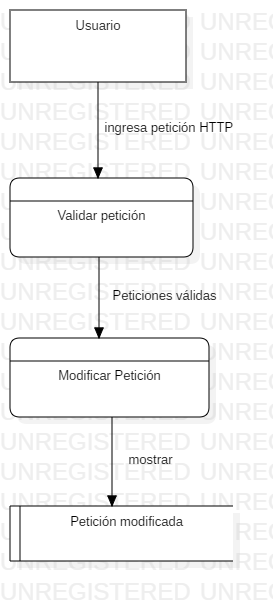
\includegraphics[width=0.5\textwidth]{imagenes/DFD_P1.png}
    			        \caption{Diagrama de flujo de datos del Prototipo 1.}
    				\end{center}
    			\end{figure}
			   
			%\subsubsection{Flujo de datos.}
			\subsubsection{Diagrama de clases.}
				\begin{figure}[!htb]
					\begin{center}
						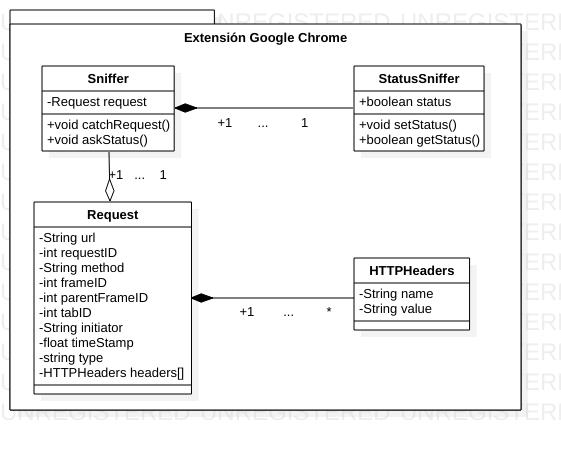
\includegraphics[width=13cm]{./imagenes/DC_P1.png}
						\caption{Diagrama de clases del Prototipo I.}
					\end{center}
				\end{figure}\newpage
				
			\subsubsection{Diagrama de secuencia.}
		    	\begin{figure}[!htb]
				    \begin{center}
			            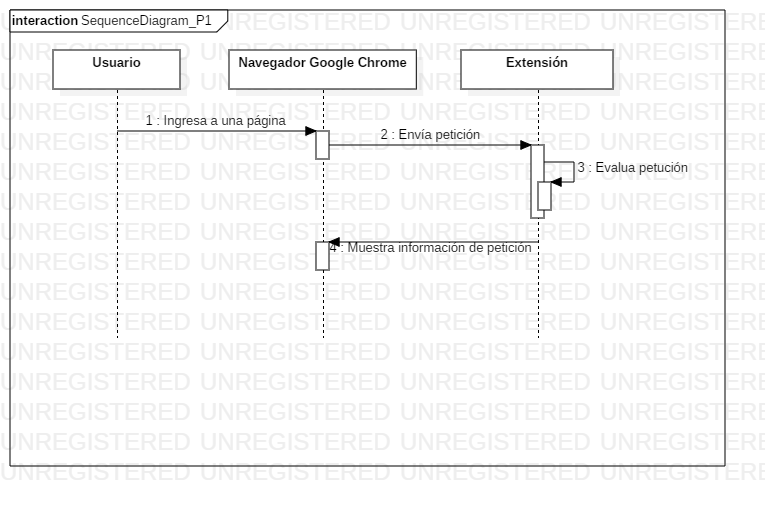
\includegraphics[width=15cm]{./imagenes/SequenceDiagram_P1.png}
				        \caption{Diagrama de secuencia del Prototipo I.}
			        \end{center}
			    \end{figure}
			\subsubsection{Interfaz de usuario.}
			\subsubsection{Requisitos de diseño.}
	%Para agregar una cita en el documento se usa \cite{refKey}, por automático los ordena conforme se van agregando
	\begin{thebibliography}{20}
	    \bibitem{ComparisonAuthenticationMethodsResources} Antonina Komarova, Alexander Menshchikov, “Comparison of Authentication Methods on Web Resources”, St. Petersburg National Research University of Information Technologies, St. Petersburg, Russia, 2016.
		\bibitem{refJavaScript} https://www.dtic.upf.edu/~tnavarrete/fcsig/javascript.pdf 
		\bibitem{refElGranLibro} https://gutl.jovenclub.cu/wp-content/uploads/2013/10/El+gran+libro+de+HTML5+CSS3+y+Javascrip.pdf
		\bibitem{refSeguridadWeb} https://www.seguridad.unam.mx/historico/documento/index.html-id=17
		\bibitem{refRoboIdentidad}
		https://www.seguridad.unam.mx/historico/documento/index.html-id=16?fbclid=IwAR0u8WAXORvBxZ3H-aMzlBhd-6o7g8ycS88eRu7nY1t1XVtCufhEcQ7hWDs
		\bibitem{refSeguridadWebAguilar} Aguilar, A. and Hernández, A. (25 de Abril de 2014). Obtenido de Sugerencias de Seguridad para Sitios Web: http://www.seguridad.unam.mx/documento-id=1143
		\bibitem{refCookies}
		https://es.wikipedia.org/wiki/Cookie\_(informatica)
		\bibitem{refCookiesPersistentes}
		http://www.allaboutcookies.org/es/galletas/cookies-persistentes-utilizados-para.html
		\bibitem{refTiposdeCookies}
		http://www.gadae.com/blog/que-son-las-cookies-tipos-de-cookies-y-como-cumplir-la-ley/
		\bibitem{refFuncionalidadCookies}
		https://www.osi.es/es/actualidad/blog/2018/07/18/entre-cookies-y-privacidad
		\bibitem{refCryptography}
		http://www.dma.fi.upm.es/recursos/aplicaciones/matematica\_discreta/web/aritmetica\_modular/criptografia.html
		\bibitem{refChaffing}
		http://www.cs.bath.ac.uk/~mdv/courses/CM30082/projects.bho/2007-8/durongdej-r-dissertation-2007-8.pdf
	\end{thebibliography}		

\end{document}

